% Options for packages loaded elsewhere
\PassOptionsToPackage{unicode}{hyperref}
\PassOptionsToPackage{hyphens}{url}
\PassOptionsToPackage{dvipsnames,svgnames,x11names}{xcolor}
%
\documentclass[
  letterpaper,
  DIV=11,
  numbers=noendperiod]{scrreprt}

\usepackage{amsmath,amssymb}
\usepackage{iftex}
\ifPDFTeX
  \usepackage[T1]{fontenc}
  \usepackage[utf8]{inputenc}
  \usepackage{textcomp} % provide euro and other symbols
\else % if luatex or xetex
  \usepackage{unicode-math}
  \defaultfontfeatures{Scale=MatchLowercase}
  \defaultfontfeatures[\rmfamily]{Ligatures=TeX,Scale=1}
\fi
\usepackage{lmodern}
\ifPDFTeX\else  
    % xetex/luatex font selection
\fi
% Use upquote if available, for straight quotes in verbatim environments
\IfFileExists{upquote.sty}{\usepackage{upquote}}{}
\IfFileExists{microtype.sty}{% use microtype if available
  \usepackage[]{microtype}
  \UseMicrotypeSet[protrusion]{basicmath} % disable protrusion for tt fonts
}{}
\makeatletter
\@ifundefined{KOMAClassName}{% if non-KOMA class
  \IfFileExists{parskip.sty}{%
    \usepackage{parskip}
  }{% else
    \setlength{\parindent}{0pt}
    \setlength{\parskip}{6pt plus 2pt minus 1pt}}
}{% if KOMA class
  \KOMAoptions{parskip=half}}
\makeatother
\usepackage{xcolor}
\setlength{\emergencystretch}{3em} % prevent overfull lines
\setcounter{secnumdepth}{5}
% Make \paragraph and \subparagraph free-standing
\makeatletter
\ifx\paragraph\undefined\else
  \let\oldparagraph\paragraph
  \renewcommand{\paragraph}{
    \@ifstar
      \xxxParagraphStar
      \xxxParagraphNoStar
  }
  \newcommand{\xxxParagraphStar}[1]{\oldparagraph*{#1}\mbox{}}
  \newcommand{\xxxParagraphNoStar}[1]{\oldparagraph{#1}\mbox{}}
\fi
\ifx\subparagraph\undefined\else
  \let\oldsubparagraph\subparagraph
  \renewcommand{\subparagraph}{
    \@ifstar
      \xxxSubParagraphStar
      \xxxSubParagraphNoStar
  }
  \newcommand{\xxxSubParagraphStar}[1]{\oldsubparagraph*{#1}\mbox{}}
  \newcommand{\xxxSubParagraphNoStar}[1]{\oldsubparagraph{#1}\mbox{}}
\fi
\makeatother

\usepackage{color}
\usepackage{fancyvrb}
\newcommand{\VerbBar}{|}
\newcommand{\VERB}{\Verb[commandchars=\\\{\}]}
\DefineVerbatimEnvironment{Highlighting}{Verbatim}{commandchars=\\\{\}}
% Add ',fontsize=\small' for more characters per line
\usepackage{framed}
\definecolor{shadecolor}{RGB}{241,243,245}
\newenvironment{Shaded}{\begin{snugshade}}{\end{snugshade}}
\newcommand{\AlertTok}[1]{\textcolor[rgb]{0.68,0.00,0.00}{#1}}
\newcommand{\AnnotationTok}[1]{\textcolor[rgb]{0.37,0.37,0.37}{#1}}
\newcommand{\AttributeTok}[1]{\textcolor[rgb]{0.40,0.45,0.13}{#1}}
\newcommand{\BaseNTok}[1]{\textcolor[rgb]{0.68,0.00,0.00}{#1}}
\newcommand{\BuiltInTok}[1]{\textcolor[rgb]{0.00,0.23,0.31}{#1}}
\newcommand{\CharTok}[1]{\textcolor[rgb]{0.13,0.47,0.30}{#1}}
\newcommand{\CommentTok}[1]{\textcolor[rgb]{0.37,0.37,0.37}{#1}}
\newcommand{\CommentVarTok}[1]{\textcolor[rgb]{0.37,0.37,0.37}{\textit{#1}}}
\newcommand{\ConstantTok}[1]{\textcolor[rgb]{0.56,0.35,0.01}{#1}}
\newcommand{\ControlFlowTok}[1]{\textcolor[rgb]{0.00,0.23,0.31}{\textbf{#1}}}
\newcommand{\DataTypeTok}[1]{\textcolor[rgb]{0.68,0.00,0.00}{#1}}
\newcommand{\DecValTok}[1]{\textcolor[rgb]{0.68,0.00,0.00}{#1}}
\newcommand{\DocumentationTok}[1]{\textcolor[rgb]{0.37,0.37,0.37}{\textit{#1}}}
\newcommand{\ErrorTok}[1]{\textcolor[rgb]{0.68,0.00,0.00}{#1}}
\newcommand{\ExtensionTok}[1]{\textcolor[rgb]{0.00,0.23,0.31}{#1}}
\newcommand{\FloatTok}[1]{\textcolor[rgb]{0.68,0.00,0.00}{#1}}
\newcommand{\FunctionTok}[1]{\textcolor[rgb]{0.28,0.35,0.67}{#1}}
\newcommand{\ImportTok}[1]{\textcolor[rgb]{0.00,0.46,0.62}{#1}}
\newcommand{\InformationTok}[1]{\textcolor[rgb]{0.37,0.37,0.37}{#1}}
\newcommand{\KeywordTok}[1]{\textcolor[rgb]{0.00,0.23,0.31}{\textbf{#1}}}
\newcommand{\NormalTok}[1]{\textcolor[rgb]{0.00,0.23,0.31}{#1}}
\newcommand{\OperatorTok}[1]{\textcolor[rgb]{0.37,0.37,0.37}{#1}}
\newcommand{\OtherTok}[1]{\textcolor[rgb]{0.00,0.23,0.31}{#1}}
\newcommand{\PreprocessorTok}[1]{\textcolor[rgb]{0.68,0.00,0.00}{#1}}
\newcommand{\RegionMarkerTok}[1]{\textcolor[rgb]{0.00,0.23,0.31}{#1}}
\newcommand{\SpecialCharTok}[1]{\textcolor[rgb]{0.37,0.37,0.37}{#1}}
\newcommand{\SpecialStringTok}[1]{\textcolor[rgb]{0.13,0.47,0.30}{#1}}
\newcommand{\StringTok}[1]{\textcolor[rgb]{0.13,0.47,0.30}{#1}}
\newcommand{\VariableTok}[1]{\textcolor[rgb]{0.07,0.07,0.07}{#1}}
\newcommand{\VerbatimStringTok}[1]{\textcolor[rgb]{0.13,0.47,0.30}{#1}}
\newcommand{\WarningTok}[1]{\textcolor[rgb]{0.37,0.37,0.37}{\textit{#1}}}

\providecommand{\tightlist}{%
  \setlength{\itemsep}{0pt}\setlength{\parskip}{0pt}}\usepackage{longtable,booktabs,array}
\usepackage{calc} % for calculating minipage widths
% Correct order of tables after \paragraph or \subparagraph
\usepackage{etoolbox}
\makeatletter
\patchcmd\longtable{\par}{\if@noskipsec\mbox{}\fi\par}{}{}
\makeatother
% Allow footnotes in longtable head/foot
\IfFileExists{footnotehyper.sty}{\usepackage{footnotehyper}}{\usepackage{footnote}}
\makesavenoteenv{longtable}
\usepackage{graphicx}
\makeatletter
\def\maxwidth{\ifdim\Gin@nat@width>\linewidth\linewidth\else\Gin@nat@width\fi}
\def\maxheight{\ifdim\Gin@nat@height>\textheight\textheight\else\Gin@nat@height\fi}
\makeatother
% Scale images if necessary, so that they will not overflow the page
% margins by default, and it is still possible to overwrite the defaults
% using explicit options in \includegraphics[width, height, ...]{}
\setkeys{Gin}{width=\maxwidth,height=\maxheight,keepaspectratio}
% Set default figure placement to htbp
\makeatletter
\def\fps@figure{htbp}
\makeatother
% definitions for citeproc citations
\NewDocumentCommand\citeproctext{}{}
\NewDocumentCommand\citeproc{mm}{%
  \begingroup\def\citeproctext{#2}\cite{#1}\endgroup}
\makeatletter
 % allow citations to break across lines
 \let\@cite@ofmt\@firstofone
 % avoid brackets around text for \cite:
 \def\@biblabel#1{}
 \def\@cite#1#2{{#1\if@tempswa , #2\fi}}
\makeatother
\newlength{\cslhangindent}
\setlength{\cslhangindent}{1.5em}
\newlength{\csllabelwidth}
\setlength{\csllabelwidth}{3em}
\newenvironment{CSLReferences}[2] % #1 hanging-indent, #2 entry-spacing
 {\begin{list}{}{%
  \setlength{\itemindent}{0pt}
  \setlength{\leftmargin}{0pt}
  \setlength{\parsep}{0pt}
  % turn on hanging indent if param 1 is 1
  \ifodd #1
   \setlength{\leftmargin}{\cslhangindent}
   \setlength{\itemindent}{-1\cslhangindent}
  \fi
  % set entry spacing
  \setlength{\itemsep}{#2\baselineskip}}}
 {\end{list}}
\usepackage{calc}
\newcommand{\CSLBlock}[1]{\hfill\break\parbox[t]{\linewidth}{\strut\ignorespaces#1\strut}}
\newcommand{\CSLLeftMargin}[1]{\parbox[t]{\csllabelwidth}{\strut#1\strut}}
\newcommand{\CSLRightInline}[1]{\parbox[t]{\linewidth - \csllabelwidth}{\strut#1\strut}}
\newcommand{\CSLIndent}[1]{\hspace{\cslhangindent}#1}

\KOMAoption{captions}{tableheading}
\makeatletter
\@ifpackageloaded{bookmark}{}{\usepackage{bookmark}}
\makeatother
\makeatletter
\@ifpackageloaded{caption}{}{\usepackage{caption}}
\AtBeginDocument{%
\ifdefined\contentsname
  \renewcommand*\contentsname{Table of contents}
\else
  \newcommand\contentsname{Table of contents}
\fi
\ifdefined\listfigurename
  \renewcommand*\listfigurename{List of Figures}
\else
  \newcommand\listfigurename{List of Figures}
\fi
\ifdefined\listtablename
  \renewcommand*\listtablename{List of Tables}
\else
  \newcommand\listtablename{List of Tables}
\fi
\ifdefined\figurename
  \renewcommand*\figurename{Figure}
\else
  \newcommand\figurename{Figure}
\fi
\ifdefined\tablename
  \renewcommand*\tablename{Table}
\else
  \newcommand\tablename{Table}
\fi
}
\@ifpackageloaded{float}{}{\usepackage{float}}
\floatstyle{ruled}
\@ifundefined{c@chapter}{\newfloat{codelisting}{h}{lop}}{\newfloat{codelisting}{h}{lop}[chapter]}
\floatname{codelisting}{Listing}
\newcommand*\listoflistings{\listof{codelisting}{List of Listings}}
\makeatother
\makeatletter
\makeatother
\makeatletter
\@ifpackageloaded{caption}{}{\usepackage{caption}}
\@ifpackageloaded{subcaption}{}{\usepackage{subcaption}}
\makeatother

\ifLuaTeX
  \usepackage{selnolig}  % disable illegal ligatures
\fi
\usepackage{bookmark}

\IfFileExists{xurl.sty}{\usepackage{xurl}}{} % add URL line breaks if available
\urlstyle{same} % disable monospaced font for URLs
\hypersetup{
  pdftitle={Getting Started with R for Economists},
  pdfauthor={Priyanga Dilini Talagala},
  colorlinks=true,
  linkcolor={blue},
  filecolor={Maroon},
  citecolor={Blue},
  urlcolor={Blue},
  pdfcreator={LaTeX via pandoc}}


\title{Getting Started with R for Economists}
\author{Priyanga Dilini Talagala}
\date{2025-01-06}

\begin{document}
\maketitle

\renewcommand*\contentsname{Table of contents}
{
\hypersetup{linkcolor=}
\setcounter{tocdepth}{2}
\tableofcontents
}

\bookmarksetup{startatroot}

\chapter*{Preface}\label{preface}
\addcontentsline{toc}{chapter}{Preface}

\markboth{Preface}{Preface}

R is a free and powerful software environment for statistical computing
and data visualization. It is widely used in academia and industry for
data analysis and research. As one of the top programming languages for
data science, R provides a variety of tools for statistical modeling,
computing, and visualization.

Since empirical research is essential in economics, programming skills
are crucial for conducting real-world data analysis. This textbook will
introduce you to R and help you develop fundamental data science skills.

\subsection*{\texorpdfstring{\textbf{About This
Book}}{About This Book}}\label{about-this-book}
\addcontentsline{toc}{subsection}{\textbf{About This Book}}

This textbook is designed for beginners, providing a strong foundation
in R for economic research. It focuses on \textbf{the tidyverse}
ecosystem, a collection of R packages that provide a simple yet powerful
approach to data analysis. You will learn how to use tidy tools to
manage and analyze data efficiently, covering the entire lifecycle of a
data science project.

\bookmarksetup{startatroot}

\chapter{Introduction to R and
RStudio}\label{introduction-to-r-and-rstudio}

\section{Installing R and Rstudio}\label{installing-r-and-rstudio}

\begin{itemize}
\item
  \textbf{Step 1:} First download R freely from the Comprehensive R
  Archive Network (CRAN) \url{https://cran.r-project.org/}. (At the
  moment of writing, R 4.4.2 is the latest version. Choose the most
  recent one.)
\item
  \textbf{Step 2:} Then install R Studio's IDE (stands for integrated
  development environment), a powerful user interface for R from
  {[}https://posit.co/download/rstudio-desktop/{]}(https://posit.co/download/rstudio-desktop/.
  Get the Open Source Edition of RStudio Desktop. RStudio allows you to
  run R in a more user-friendly environment.

  \begin{itemize}
  \item
    You need to install \textbf{both} R and Rstudio to use RStudio.
  \item
    If you have a pre-existing installation of R and/or RStudio, I
    highly recommend that you reinstall both and get as current as
    possible.
  \end{itemize}
\item
  \textbf{Step 3:} Then open \textbf{Rstudio}.
\end{itemize}

\subsection{Posit Cloud}\label{posit-cloud}

\begin{itemize}
\item
  In 2022, RStudio changed its corporate name to Posit with the aim of
  expanding its focus beyond R to include users of Python and Visual
  Studio Code.
\item
  If you don't want to download or install R and R Studio, you can use
  RStudio on \hyperref[posit-cloud]{Posit Cloud} (https://posit.cloud/)
  for free.
\end{itemize}

\section{RStudio layout}\label{rstudio-layout}

The RStudio interface consists of four panes: See Figure 1)

\begin{enumerate}
\def\labelenumi{\arabic{enumi}.}
\item
  \textbf{Source pane}
\item
  \textbf{Console pane}
\item
  \textbf{Environment pane}, containing the Environment, History,
  Connections, Build, and Tutorial tabs
\item
  \textbf{Output pane}, containing the Files, Plots, Packages, Help,
  Viewer, and Presentation tabs
\end{enumerate}

\begin{center}
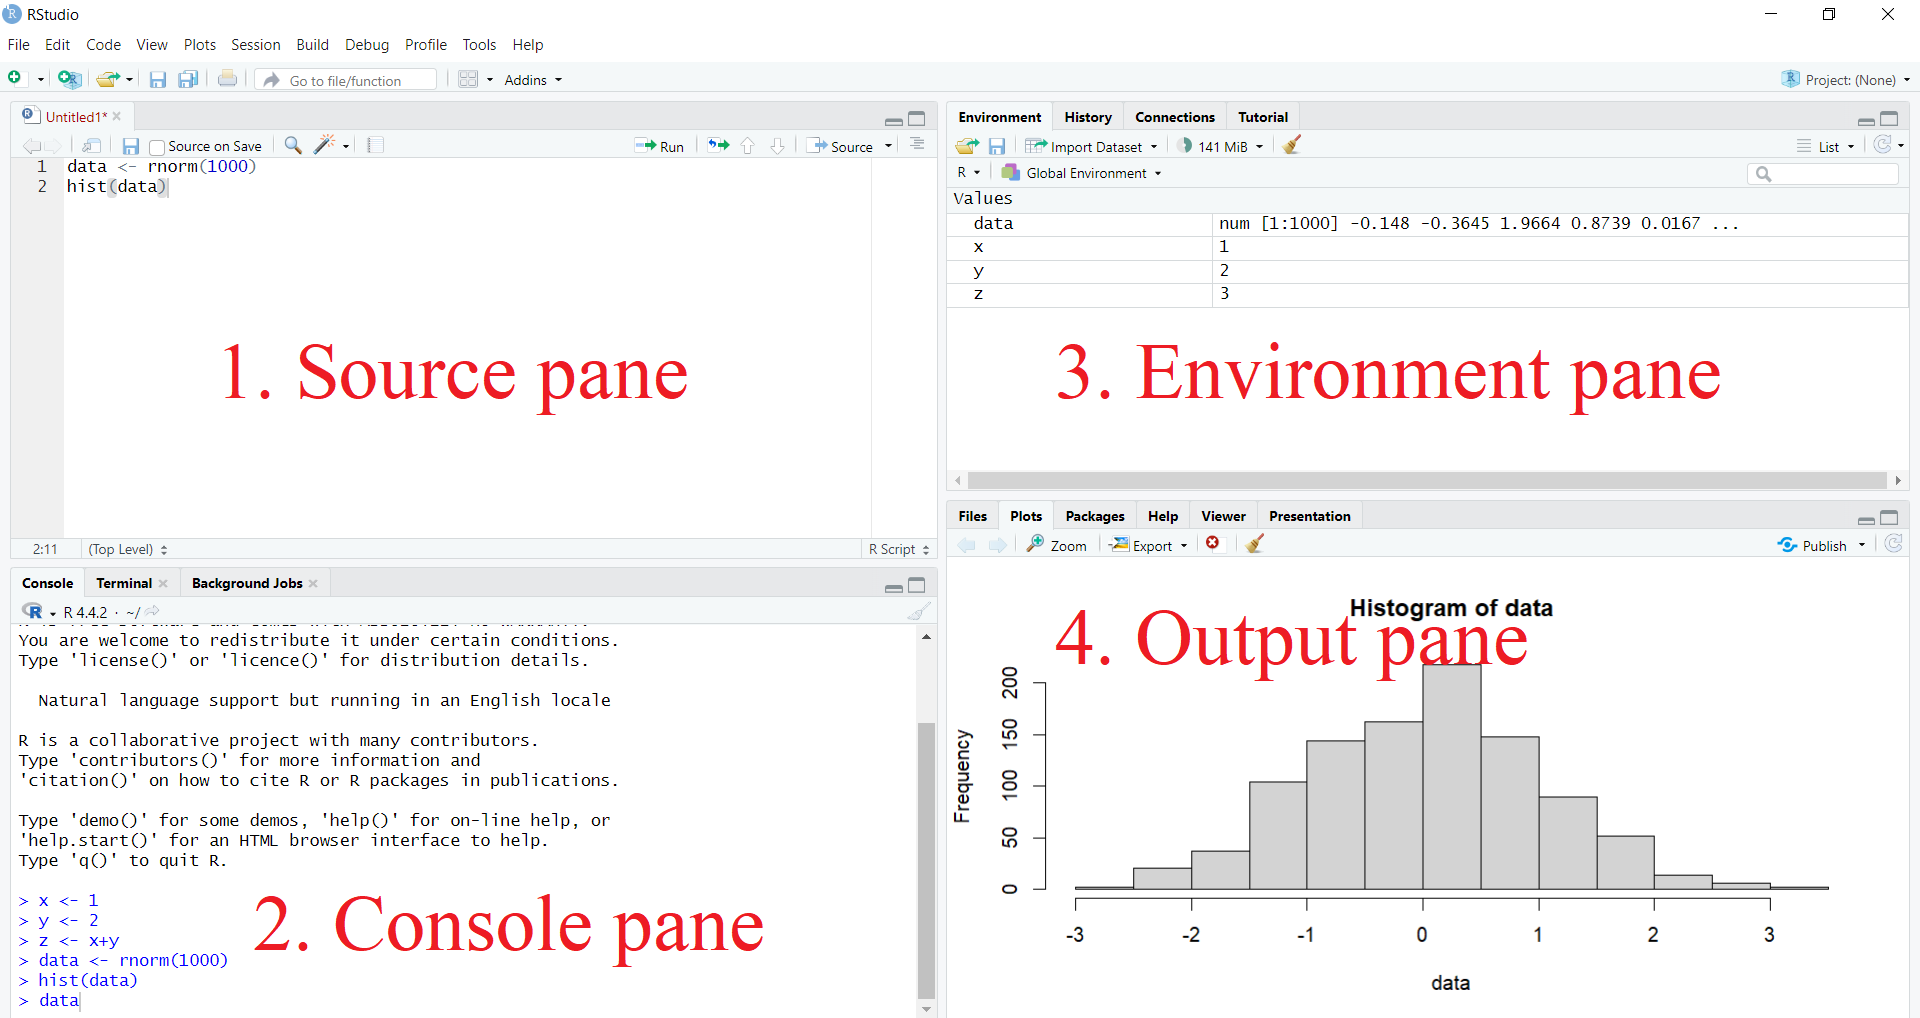
\includegraphics[width=1\textwidth,height=\textheight]{fig/1_Rstudio_Layout.png}
\end{center}

\subsection{Console Pane}\label{console-pane}

\begin{itemize}
\item
  This is where you type and execute all your R commands.
\item
  You can enter R commands after the `\textgreater{}' prompt, and R will
  process and execute them.
\item
  This is the most essential window, as it is where R performs
  computations and executes your instructions.
\end{itemize}

\subsection{Source pane}\label{source-pane}

\begin{itemize}
\item
  In this window, a collection of commands (scripts) can be edited and
  saved.
\item
  If this window is not visible, you can open it via File → New File → R
  Script.
\item
  Simply typing a command in the Source pane is not enough; it must be
  sent to the Console before R executes it.
\item
  To run a line from the Source pane, place your cursor on the desired
  line or select multiple lines to execute, then click Run or press CTRL
  + ENTER to send them to the Console pane.
\item
  Make sure to save the `Untitled1' file as a \texttt{*.R} script.
\end{itemize}

\subsection{Environment pane}\label{environment-pane}

\begin{itemize}
\tightlist
\item
  This window contains multiple tabs: Environment, History, Connections,
  Build, and Tutorial.
\end{itemize}

The Environment tab displays all active objects.

\begin{itemize}
\item
  For data frames, clicking the grid symbol opens the full data frame in
  the Source pane.
\item
  The History tab shows previously typed commands.
\item
  To send a command in the history tab to the Source pane, select it and
  click the ``To Source'' icon, or click ``To Console'' to execute it in
  the Console.
\end{itemize}

\subsection{Output Pane}\label{output-pane}

\begin{itemize}
\item
  This window contains multiple tabs: Files, Plots, Packages, Help,
  Viewer, and Presentation.
\item
  It allows you to open files, view plots (including previous ones),
  install and load packages, access help functions, and display web
  content such as Shiny apps and Quarto-generated web pages.
\end{itemize}

Now you are familiar with the layout. Let's begin with R basics.

\section{Installing an R Package}\label{installing-an-r-package}

\begin{itemize}
\item
  The primary source for R packages is CRAN (Comprehensive R Archive
  Network).
\item
  Packages can be installed using the \texttt{install.packages()}
  function in R.
\item
  To install a single package, pass its name as the first argument to
  \texttt{install.packages()}.
\item
  The following code installs the tidyverse package from CRAN:
\end{itemize}

\begin{Shaded}
\begin{Highlighting}[]
\FunctionTok{install.packages}\NormalTok{(}\StringTok{"tidyverse"}\NormalTok{)}
\end{Highlighting}
\end{Shaded}

\begin{itemize}
\item
  This command downloads and installs the \texttt{tidyverse} package
  from CRAN.
\item
  Any dependencies required by the package will also be downloaded and
  installed.
\item
  Installing the tidyverse package may take several minutes, but you
  only need to do this once. Think of it like installing a mobile
  app---you install it once on your smartphone and can use its features
  until a new version is released, at which point you may need to update
  it
\end{itemize}

\subsection{Alternative way to install R packages in
Rstudio}\label{alternative-way-to-install-r-packages-in-rstudio}

\begin{itemize}
\item
  An alternative way to install R packages is through the Packages tab
  in the Output Pane.
\item
  Navigate to the Packages tab in the Output Pane and click Install.
\item
  Under ``Install from,'' select ``Repository (CRAN)''.
\item
  In the Packages field, enter the name of the package you want to
  install.
\item
  To install multiple packages at once, separate the package names with
  commas.
\item
  Finally, click Install.
\end{itemize}

\begin{center}
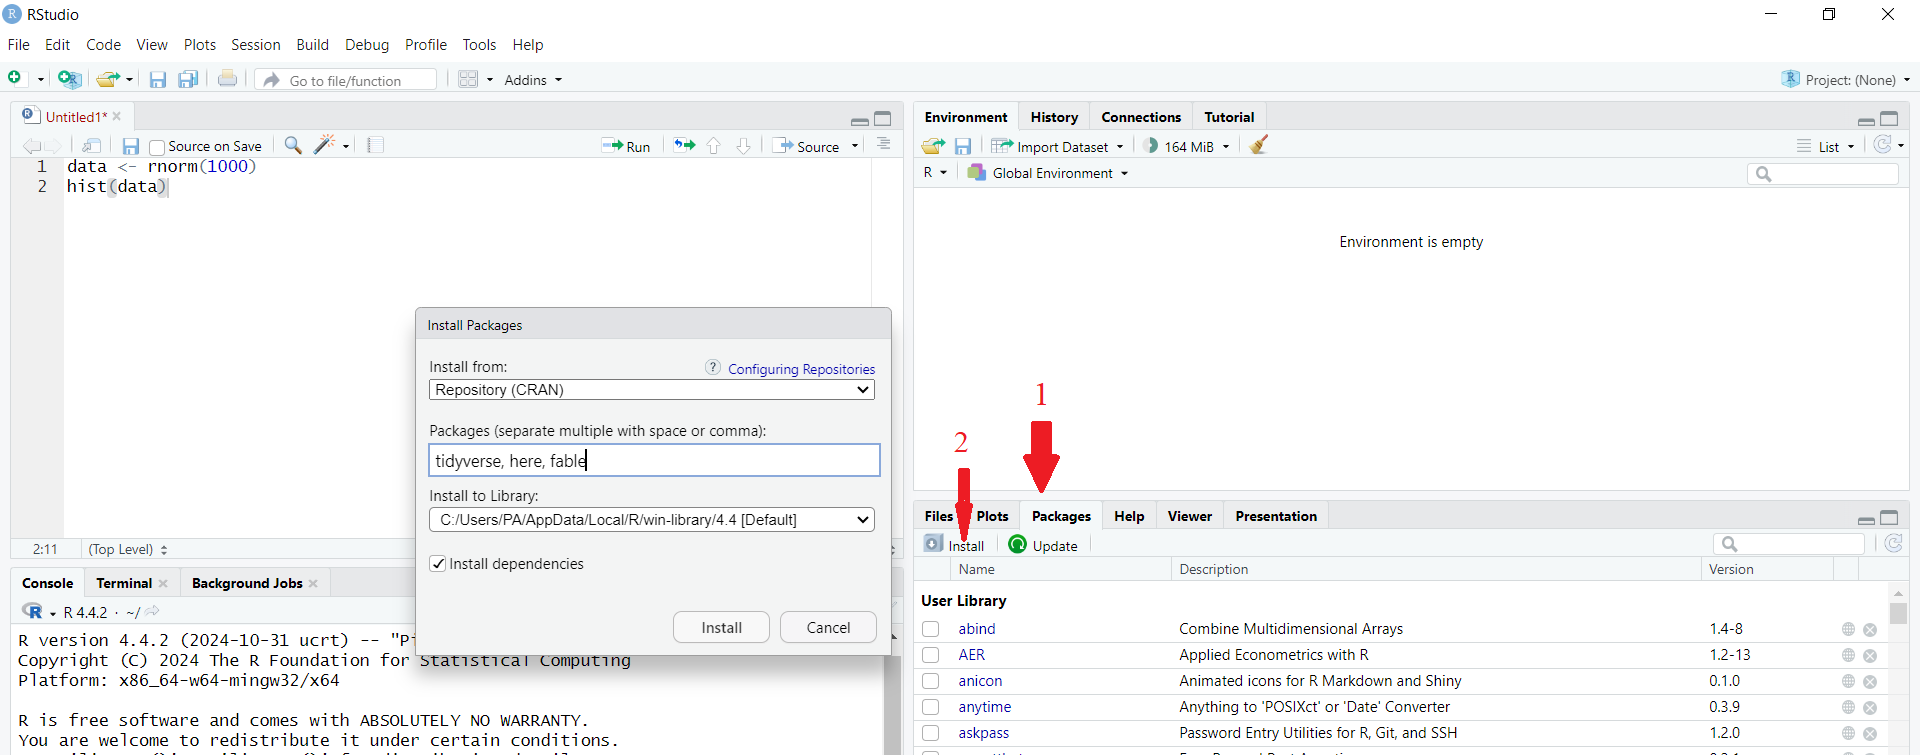
\includegraphics[width=1\textwidth,height=\textheight]{fig/2_install_packages.png}
\end{center}

\section{Loading an R Package}\label{loading-an-r-package}

\begin{itemize}
\item
  Installing a package does not automatically make it available for use;
  you must load it. It's like a mobile app---you need to open it to
  access its functionalities.
\item
  The \texttt{library()} function is used to load installed packages
  into R.
\item
  To load the tidyverse package, use:
\end{itemize}

\begin{Shaded}
\begin{Highlighting}[]
\FunctionTok{library}\NormalTok{(tidyverse)}
\end{Highlighting}
\end{Shaded}

\begin{verbatim}
-- Attaching core tidyverse packages ------------------------ tidyverse 2.0.0 --
v dplyr     1.1.4     v readr     2.1.5
v forcats   1.0.0     v stringr   1.5.1
v ggplot2   3.5.1     v tibble    3.2.1
v lubridate 1.9.3     v tidyr     1.3.1
v purrr     1.0.2     
-- Conflicts ------------------------------------------ tidyverse_conflicts() --
x dplyr::filter() masks stats::filter()
x dplyr::lag()    masks stats::lag()
i Use the conflicted package (<http://conflicted.r-lib.org/>) to force all conflicts to become errors
\end{verbatim}

\begin{itemize}
\item
  \textbf{Note: Do not put the package name in quotes when using
  library().}
\item
  Some packages display messages when loaded, while others do not.
\end{itemize}

\section{Getting Started with R}\label{getting-started-with-r}

For a detailed introduction to R, refer to:

\href{https://cran.r-project.org/doc/manuals/R-intro.pdf}{An
Introduction to R: https://cran.r-project.org/doc/manuals/R-intro.pdf}

\bookmarksetup{startatroot}

\chapter{R Programming Basics}\label{r-programming-basics}

\bookmarksetup{startatroot}

\chapter{Reproducible Reporting with
Quarto}\label{reproducible-reporting-with-quarto}

\bookmarksetup{startatroot}

\chapter{Data Import and Export}\label{data-import-and-export}

\bookmarksetup{startatroot}

\chapter{Reproducible Reporting with
Quarto}\label{reproducible-reporting-with-quarto-1}

\bookmarksetup{startatroot}

\chapter{Data Wrangling}\label{data-wrangling}

\bookmarksetup{startatroot}

\chapter{Data Visualization}\label{data-visualization}

\bookmarksetup{startatroot}

\chapter{Introduction to Statistical
Modelling}\label{introduction-to-statistical-modelling}

\bookmarksetup{startatroot}

\chapter*{References}\label{references}
\addcontentsline{toc}{chapter}{References}

\markboth{References}{References}

\phantomsection\label{refs}
\begin{CSLReferences}{0}{1}
\end{CSLReferences}




\end{document}
